\chapter{Student marks}\label{ap:marks}

Student attainment is quantified through the marks they are awarded. While this is not a perfect metric for assessing student learning \citep[cf.][chapter 11]{Ramsden1992}, it provides an excellent starting point. Here, I examine the essay marks for my students. Since I only have a small sample size, it is not possible to draw definite conclusions. However, checking the marks for patterns can still be informative. The marks do not necessarily reflect how much students learnt from essay writing, since they necessarily do not include the impact of receiving feedback on the final essay.

In \secref{marks-students} I introduce the group of students whose marks I am analysing. I include last year's students for comparison. Results are presented and analysed in \secref{plots}. We conclude with a summary in \secref{marks-end}.

\section{Student sample}\label{sec:marks-students}

We shall examine the marks of of my students from 2013/2014 and 2014/2015. The 2014/2015 students are described in \secref{2014-15students}, again the student who joined part-way through the year will be excluded from the analysis as they have a different experience of the year. In 2013/2014 I had eight students, again divided into two groups. One was an affiliate student on an interstitial year from a non-UK university. I have excluded their results from the analysis because they have had a different educational history from the University of Birmingham students; additionally, they have different motivations as they only need to pass the year for their degree. Of the remaining students, one was female, none were international, and none had disclosed special educational needs. First-year results ranged from 2.ii to (low) 1st. The two cohorts of students are roughly comparable, although not exactly equivalent.

\section{Marks \& discussion}\label{sec:plots}

The essay marks are awarded on a scale from $0$ to $100$ according to the mark scheme explaining in \secref{problem}. None of the students were docked marks for being late or over the word limit. Some students scored under $60$, necessitating the need to resubmit. Here, we will only consider the mark from their first attempt to make the comparison fair.

The distribution of essay marks are shown in \figref{marks}. To make the data easier to visualise, individual results have been smoothed with a Gaussian kernel: the total distribution is constructed by summing a series of Gaussian distributions, with each centred on the mark of an individual student. This gives the ordinate axis the peculiar units of students per mark, as integrating the area under the curves will give the total number of students (seven for 2013--2014 and eight for 2014--2015).\footnote{The Gaussians have been renormalised such that integrating between $0$ and $100$ (the range of possible marks) gives unity, although this makes a negligible change for the distributions considered here.} The standard deviation of the Gaussian is $\sqrt{10}~\mathrm{marks}$, chosen assuming that each of the ten mark-scheme categories has an associated uncertainty of $\pm1$; this is probably an overestimate, but will suffice for our purpose of qualitatively examining the data. The 2013/2014 results show a bimodal distribution with a clear outlier. One student took particular interest in the essay, and did an excellent job of using all the advice I gave them. The 2014/2015 results also show a bimodal distribution. Marks typically fall in the range $60$--$80$.
\begin{figure}
  \centering
   \subfigure[{2013/2014}]{\label{fig:2013-marks} \includegraphics[width=0.47\textwidth]{./figs/Fig_2013_marks}} \quad
   \subfigure[{2014/2015}]{\label{fig:2014-marks} 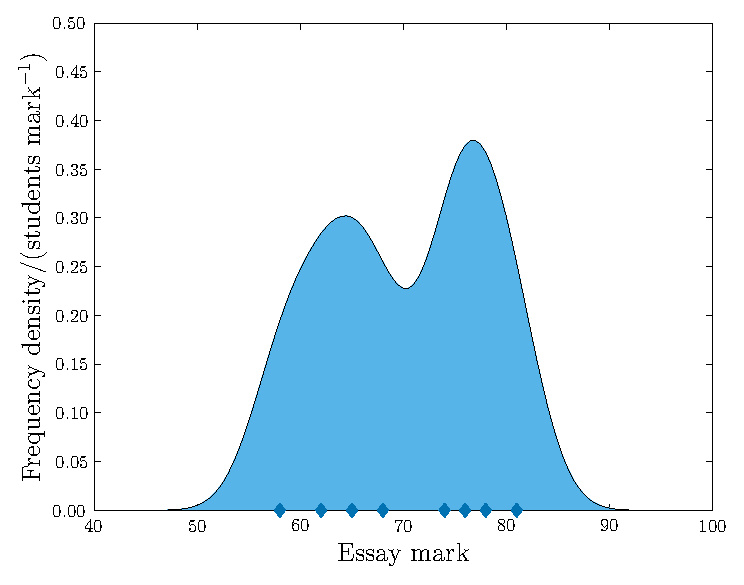
\includegraphics[width=0.47\textwidth]{./figs/Fig_2014_marks}}  
\caption{Distribution of essay marks for both cohorts of students. The diamonds indicate the actual marks; the frequency densities have been constructed by smoothing with a Gaussian kernel with a standard deviation of $\sqrt{10}~\mathrm{marks}$. The mean mark of the 2013/2014 students is $(68.1\pm3.4)~\mathrm{marks}$, and the mean for 2014/2015 students is $(70.3\pm2.7)~\mathrm{marks}$, where the uncertainties quoted on the means are estimated from the standard errors \citep[chapter 22]{Mackay2003}.}
  \label{fig:marks}
\end{figure}

Before we can draw conclusions from the distribution marks, it is necessary to consider the aptitudes of the students. Ideally, we would like to compare with marks from their first-year essays, to assess progress. I do not have access to these. However, I do have their average mark from first-year (a mark between $0$ and $100$). We would expect this to be correlated with their second-year essay mark. In \figref{diff}, we plot the distribution of differences between essay marks and their first-year averages.\footnote{Using relative difference instead of absolute difference gives qualitatively similar distributions.} We use the same Gaussian smoothing as in \figref{marks}. The 2013/2014 distribution shows a bimodal structure, with some students doing better than expected on their essay and others doing worse. The division is not related to tutorial group. There is no clear outlier (the high scoring student from \figref{2013-marks} has been absorbed into the better-than-expected peak). The 2014/2015 distribution is more consistent with expectations; the bimodality seen in \figref{marks} is an artefact of having two groups of different abilities.
\begin{figure}
  \centering
   \subfigure[{2013/2014}]{\label{fig:2013-diff} \includegraphics[width=0.47\textwidth]{./figs/Fig_2013_mark_diff}} \quad
   \subfigure[{2014/2015}]{\label{fig:2014-diif} \includegraphics[width=0.47\textwidth]{./figs/Fig_2014_mark_diff}}  
\caption{Distribution of difference between essay and average first-year marks for both cohorts of students. The diamonds indicate the actual mark differences; the frequency densities have been constructed by smoothing with a Gaussian kernel with a standard deviation of $\sqrt{10}~\mathrm{marks}$. A positive difference indicates the student did better on the essay than in first year. The mean mark difference of the 2013/2014 students is $(2.7\pm4.3)~\mathrm{marks}$, and the mean for 2014/2015 students is $(2.1\pm2.0)~\mathrm{marks}$. Averaging across both cohorts, the mean mark difference is $(2.4\pm2.3)~\mathrm{marks}$. The uncertainties quoted on the means are estimated from the standard errors.}
  \label{fig:diff}
\end{figure}

The difference between the two years is striking, but we are dealing with small sample sizes. In 2013/2014 I had one student who took special interest in the essay, and another who took no interest in revision and so underperformed in exams; the factors can go some way towards accounting for the over-performance in the essay compared to first year. Equally, I had one student who misjudged the level of rigour needed in an essay and performed worse than I expected given their enthusiasm and scientific ability.\footnote{They resubmitted and their second mark was more consistent with their first-year mark. The difference after remarking was $-5~\mathrm{marks}$ and I suspect further that improvement would have been achieved if they were not conscious of the cap at $60~\mathrm{marks}$.} In 2014/2015 I had students who achieved higher marks in first-year, it is much more difficult for them to achieve a significantly higher mark in their essays, so one might expect the differences to taper off. Without a larger population of results, we must be cautious in drawing conclusions.

While it is possible to explain away differences, this does neglect the fact that there will always be a range of student abilities and motivations. Teaching must take this diversity into account. In \figref{mark-mark-diff}, we further examine the difference between the essay and first-year marks. In 2014/2015 there is no obvious correlation between the mark difference and performance in the essay, this is not the case in 2013/2014. Those who did well seem to show significant improvement compared to first year, while those who did badly show under-performance, although the two clusters overlap in terms of essay mark. This is evidence of my 2013/2014 teaching having a polarising effect: those who were able to assimilate it went on to perform well, but those who were unable performed badly. In 2014/2015, my teaching of essay writing was more evenly distributed throughout the year (see \secref{essay-methods}), and involved a greater variety of methods; this may have made it more accessible and easier to digest, benefiting a greater selection of students. However, in distributing the teaching, it seems to have lost some of its impact, and there is not as great an increase in marks. Moving some of the discussion to the Autumn term, may have diluted the impact of giving advice while the essay was being written. It appears that there are potentially advantages and disadvantages to the adaptations I made to my teaching schedule.
\begin{figure}
  \centering
   \includegraphics[width=0.6\textwidth]{./figs/Fig_mark_mark_diff}
\caption{Difference between essay and average first-year marks as a function of essay marks. The red--orange squares are the results for the 2013/2014 students and the light blue circles are for the 2014/2015 students. The 2013/2014 appear to fall into two clusters: those with positive mark differences and those with negative mark differences. The mean essay mark for the positive-difference group is $(73.3\pm4.5)~\mathrm{marks}$, and the mean for the negative-difference group is $(61.3\pm1.4)~\mathrm{marks}$, where the uncertainties quoted are estimated from the standard errors.}
  \label{fig:mark-mark-diff}
\end{figure}

There is one further statistic that can be incorporated into our analysis, tutorial attendance. We would expect attendance to be correlated with attainment. First, there is a causal link: those who spend more time engaging with educational activities should see a greater benefit from them. Second, attendance can be linked to motivation, which is correlated with learning \citep[e.g.,][chapter 4]{Ramsden1992}. Absence from tutorial could be because of apathy or disorganisation (see \secref{other-discuss}); because of poor health or personal matters, or because a clash with another educational activity such as an extracurricular or careers event. The first set of reasons indicates a lack of engagement with or low-prioritisation of their studies, which would be correlated with poor attainment. The second set does indicate anything about how the student views the subject or their studies, but may still be linked to a lack of motivation as a side effect of potentially depressing problems. The final set may indicate that the student is positively engaged in their studies, taking an active interest in the subject or their own achievement; this may indicate good attainment if this benefit outweighs the disadvantage of missing teaching sessions. In \figref{attend} we plot fractional attendance for year (the $20$ tutorials) against essay mark. There is no obvious correlation for 2013/2014, but there does appear to be the expected positive trend for 2014/2015.
\begin{figure}
  \centering
   \includegraphics[width=0.6\textwidth]{./figs/Fig_attend}
\caption{Essay mark as a function of tutorial attendance. The red--orange squares are the results for the 2013/2014 students and the light blue circles are for the 2014/2015 students. There are $20$ tutorials, hence attendance is quantized into divisions on $0.05$.}
  \label{fig:attend}
\end{figure}

The difference between the cohorts could again be attributed to the small sample sizes; however, it may also trace the difference in teaching. In 2013/2014, teaching of essay writing was concentrated to tutorials 12 and 14 (see \tabref{2013-14}). Attendance at these two sessions was perfect. Hence no students suffered from missing an important lesson. The second-order effect of the impact of motivation (as traced by attendance) on performance appears to be negligible. In 2014/2015, teaching of communication skill was distributed throughout the year, making any given absence more significant. If we only consider the main essay-writing tutorials 3, 12, 13 and 14 (\tabref{2014-15}), the trend persists.  One student attended half of these tutorials and received an essay mark of $62~\mathrm{marks}$; two attended three out of four and received a mean mark of $(67.0\pm6.4)~\mathrm{marks}$, and the remaining five attended all four and have an mean mark of $(73.2\pm2.7)~\mathrm{marks}$. The quoted uncertainties on the means have been estimated from the standard error \citep[chapter 22]{Mackay2003}. Attendance appears to correlate with performance as being absent from tutorial means that students miss useful teaching. The provision of written materials, like a blog (\secref{blog}), that can be studied any time may ameliorate the impact of missing tutorial, but only if students are aware of their existence and importance. Breaking up teaching across multiple tutorials increases the probability that one or more sessions will be missed; however, it also reduces the probability that all of the teaching on essay writing is missed, which would likely be extremely detrimental.

\section{Summary \& conclusion}\label{sec:marks-end}

From the limited data available, we may draw some provisional qualitative conclusions on the effectiveness of teaching. Making more robust statements would require a more sophisticated analysis or further data. Unsurprisingly, our data suggest that essay-writing ability is correlated both with overall proficiency (measured by average first-year mark) and attendance at tutorials where essay writing was discussed. Comparing the two cohorts, it appears that the more distributed teaching of 2014/2015 is safer. Students are less likely to under-perform and there is a lower risk of missing all the relevant teaching. However, the teaching of 2013/2014 was more effective at inspiring significant over-performance (compared to the first-year mark). This may be because a concentrated session during the Spring term is particularly effective, as students can immediately make use of the information, but we do not have the evidence to prove this. We conclude, that neither the teaching of 2013/2014 nor 2014/2015 is superior to the other in all regards.
